\section{Theorie}
Im thermischen Gleichgewicht bei einer Temperatur $T$ gilt zwischen den Besetzungszahlen
$N_{1}$ und $N_{2}$ zweier Energieniveaus $W_{1}$ und $W_{2}$ der äußeren Elektronenschalen
die Boltzmann-Gleichung
\begin{equation}
  \frac{N_2}{N_1} = \frac{g_2}{g_1} \frac{\exp\left(- \frac{W_2}{kT}\right) }{\exp\left(- \frac{W_1}{kT}\right) }.
  \label{Theo:eq1}
\end{equation}
Die statischen Gewichte $g_{1}$ und $g_{2}$ geben hierbei an, wie viele Zustände
im zugehörigen Energieniveau möglich sind.
Die Vergleichsrelation zwischen $N_{1}$ und $N_{2}$ ist im thermischen Ggw. derer zwischen
$W_{1}$ und $W_{2}$ entgegengesetzt, aus $W_{1} < W_{2}$ folgt also $N_{1} > N_{2}$,
dennoch könnnen hier Abweichungen auftreten.
Dazu wird die Methode des optischen Pumpens genutzt.
Hiermit lassen sich Änderungen am durch die Boltzmann Gleichung \eqref{Theo:eq1}
vorgegebenen Verhältnis bis zur Inversion der Vergleichsrelation zwischen
$N_{1}$ und $N_{2}$ hervorrufen.
Die resultierende Verteilung ist nicht thermisch und ermöglicht das Induzieren von
Strahlungsübergängen zwischen dem im obrigen Beispiel
energetisch ungünstigeren, aber im Inversionsfall
dennoch stärker besetztem, Zustand $W_{2}$ und dem energetisch günstigeren Zustand
$W_{1}$, sodass ein Photon der Energie
\begin{equation}
  h\nu = W_{2} - W_{1}
\end{equation}
emittiert oder absorbiert wird.
Eine Messung dieser Photonen ermöglicht nun Aussagen über die zugrundeliegenden
Niveauunterschiede.
Diese können beispielsweise durch Hyperfeinstruktur- oder Zeeman-Aufspaltung
in einem Magnetfeld bedingt sein.
Aufgrund des geringen Energieunterschiedes zwischen Energieniveaus in diesen Fällen
liegt die Energie der emittierten Photonen weit unter der thermischen Energie $\propto kT$
des Systems, sodass Messungen mit hoher Präzision möglich sind.

\subsection{Der Zeeman-Effekt}
Dem Zeeman-Effekt, benannt nach seinem Entdecker \textsc{Pieter Zeeman},
liegt die Kopplung der Drehimpulse der Hüllenelektronen
zugrunde.
Zu Unterscheiden ist hier zwischen dem normalen und dem annormalen Zeeman-Effekt.
Der normale Zeeman-Effekt tritt auf, wenn Atome mit abgeschlossenen Schalen untersucht
werden.
In diesem Fall kompensieren sich alle Drehimpulse.
Im Allgemeinen ist dies natürlich nicht der Fall, sodass der annormale Zeeman-Effekt,
der beispielsweise bei Wasserstoff und den Alkali-Metallen auftritt, betrachtet werden muss.
Die Bahndrehimpulse $\vec{L}$ und Spins $\vec{S}$ der Elektronen koppeln dabei
zu einem Gesamtdrehimpuls $\vec{J}$, der über das Bohrsche Magneton $\mu_{\symup{B}}$
und den Lande-Faktor $g_{\symup{J}}$ durch
\begin{equation}
  \vec{\mu}_{\symup{J}} = - g_{\symup{J}} \mu_{\symup{B}} \vec{J} \quad ; \quad
  |\vec{\mu}_{\symup{J}}| = - g_{\symup{J}} \mu_{\symup{B}} \sqrt{J(J+1)}
  \label{Theo:eq2}
\end{equation}
mit einem magnetischen Moment verknüpft ist.
Das magnetische Gesamtdrehimpulsmoment bestimmt sich dabei aus den analog nach \eqref{Theo:eq2}
bestimmten magnetischen Momenten von Bahndrehimpuls und Spin durch
\begin{equation}
  \vec{\mu}_{\symup{J}} = \vec{\mu}_{\symup{L}} + \vec{\mu}_{\symup{S}}.
\end{equation}
Mit den Lande-Faktoren $g_{\symup{L}} = 1$ und $g_{\symup{S}} = \num{2.00232}$ und
der Drehimpulsaddition folgt
\begin{equation}
  g_{\symup{J}} = \frac{3,0023J(J+1) + 1,0023(S(S+1) - L(L+1))}{2J(J+1)},
  \label{eqn:gJ}
\end{equation}
sodass in einem Magnetfeld $B$ eine Niveauaufspaltung in $2J+1$ Niveaus der Energie
\begin{equation}
  U_{\symup{mag}} = m_{\symup{J}} g_{\symup{J}} \mu_{\symup{B}} B \quad \text{mit} \quad m_{\symup{J}} \in [-J,-J+1,...,J-1,J]
  \label{Theo:eq3}
\end{equation}
beobachtet werden kann.
Dies wird als Zeeman-Effekt bezeichnet. Im Fall einer Hyperfeinstrukturaufspaltung
muss dies noch modifiziert werden.

\subsection{Die Hyperfeinstrukturaufspaltung}
Besitzt das beobachtete Atom nun noch einen von Null verschiedenen Kernspin $\vec{I}$,
so koppelt dieser, ausreichend kleine äußere Magnetfelder vorrausgesetzt, mit dem
Gesamtdrehimpuls der Hüllenelektronen zum Gesamtdrehimpuls des Atoms
\begin{equation}
  \vec{F} = \vec{J} + \vec{I}.
  \label{eqn:F-Vektor}
\end{equation}
Auch hier ist wieder eine diskrete Anzahl an Werten für die Aufspaltung möglich.
Die zugehörige Quantenzahl $F$ hat einen Wertevorrat von $I+J$ bis $|I-J|$ in ganzzahligen
Schritten, umfasst also $2j+1$ Werte für den Fall, dass $J<I$ und $2I+1$ Werte für
$J>I$.
Im Falle eines nicht verschwindenden Kernspins tritt nicht die im vorherigen
Kapitel beschriebene Zeeman-Aufspaltung mit $m_{\symup{J}} \in [-J,-J+1,...,J-1,J]$
auf.
Die Quantenzahl $m_{\symup{J}}$ muss hier durch $m_{\symup{F}} \in [-F,-F+1,...,F-1,F]$ ersetzt werden.
Auch die Energien der Aufspaltung in \eqref{Theo:eq3} muss angepasst werden.
Diese beträgt nun
\begin{equation}
  U_{\symup{HF}} = g_{\symup{F}} \mu_{\symup{B}} B
  \label{Theo:eq4}
\end{equation}
ersetzt werden. Der zugehörige Lande-Faktor $g_{\symup{F}}$ berechnet sich nach
eine ähnlichen Ansatz wie oben zu
\begin{equation}
  g_{\symup{F}} = g_{\symup{J}} \frac{F(F+1) + J(J+1) - I(I+1)}{2F(F+1)}.
  \label{eqn:gF}
\end{equation}
Für stärkere Magnetfelder muss der Abstand zwischen den Zeeman-Niveaus \eqref{Theo:eq4} um
Terme höherer Ordnung ergänzt werden.
Erst hier wird die Aufspaltung von $m_{\symup{F}}$ abhängig:
\begin{equation}
  U_{\symup{HF}} = g_{\symup{F}} \mu_{\symup{B}} B + (g_{\symup{F}} \mu_{\symup{B}} B)^{2} \frac{1-2m_{\symup{F}}}{\symup{\Delta}E_{\symup{HF}}} \, ,
  \label{eqn:quadratischer-zeeman}
\end{equation}
wobei $\symup{\Delta}E_{\symup{HF}}$ den Absatnd zwischen dem zu $F$ und $F+1$ gehörigen
Niveau der Hyperfeinstrukturaufspaltung bezeichnet.

\subsection{Optisches Pumpen}
In Atomen können nun verschiedene Übergänge zwischen Zeeman-Niveaus identifiziert werden,
die den Auswahlregeln $\symup{\Delta} m_{J} = 0,\, \pm 1$ gehorchen.
Erstere werden dabei als $\pi$-Übergänge bezeichnet und emittieren
parrallel zum Magnetfeld, linear polarisiertes Licht.
Die beiden verbleibenden $\sigma^{\pm}$-Übergänge emittieren zusätzlich in Richtung
des Magnetfeldes rechts- ($\sigma^{+}$) oder links-zirkular ($\sigma^{-}$) polarisiertes Licht.
Wird nun eine Probe mit Licht von geeigneter Polarisierung und Energie bestrahlt
kann ausgewählt werden, welche Hüllenelektronen in welches Energieniveau
gehoben werden sollen.
Die angeregten Hüllenelektronen gehen nach kurzer Zeit wieder in ihren Grundzustand über.
Da nun aber auch der Grundzustand aufgrund der Zeeman-Aufspaltung mehrere Unterniveaus
besitzt, von denen nur Elektronen eines ausgewählten Niveaus angeregt wurden,
welche aber alle im Zuge der Abregung (wieder) von Elektronen bevölkert werden,
lehrt sich das durch das eingestrahlte Licht ausgewählte Niveau zum Vorteil
der anderen.
Dieser Inversionsprozess kann durch Beobachtung des den Versuchsaufbau durchquerenden
Lichtes beobachtet werden.
Solange sich noch Elektronen im anfangs ausgewählten Energieniveau befinden,
erscheint das Medium für das einfallende Licht anfangs stärker, später schwächer opak.
Sind alle Elektronen in ein höheres Niveau gepumpt, wird es lichtdurchlässig.
Als Lichtquelle kommen insbesondere Spektrallampen infrage.
Hierbei sind die Energieverteilungen breiter als die beobachtete Differenz zwischen
Zeeman-Niveaus, sodass die benötigte Energie vorhanden ist.

\subsubsection{Optisches Pumpen als Messmethode}
In den vorherigen Überlegungen wurde immer von spontaner Emission ausgegangen.
Dies ist nun die einzige Möglichkeit einen Übergang zwischen zwei Energieniveaus
zu erhalten.
Die zweite Möglichkeit liegt in der induzierten Emission, bei der durch Einstrahlung
eines Photons, dessen Energie der des Übergangs entspricht, der Übergang erzwungen wird.
In diesem Fall erhält man zwei Photonen der Übergangsenergie.
Es lässt sich zeigen, dass die Wahrscheinlichkeit zur spontanen Emission $\propto \nu^{3}$
ist und im Energiebereich der Zeeman-Aufspaltung weit unter der Wahrscheinlichkeit
für induzierte Emission liegt.
Letztere kann daher genutzt werden, um Zeeman-Niveaus auszumessen.
Wird dabei zuerst durch optisches Pumpen ein Niveau entlehrt und damit der Versuchsaufbau für das eingestrahlte
Licht durchsichtig, kann durch Anlegen eines Magnetfeldes der Punkt erreicht werden,
an dem induzierte Emission einsetzt.
Dies ist der Fall, wenn
\begin{equation}
  B = \frac{4 \pi \m}{e g_{\symup{J}}}\nu
\end{equation}
ist.
Es setzt die Entlehrung des vorher angereicherten Niveaus ein und der Versuchsaufbau wird wieder
opak, die beobachtete Resonanz eignet sich also zum ausnessen des Übergangs.
Wird das Magnetfeld weiter erhöht, bleibt die induzierte Emission aus und es setzt
wieder eine Inversion durch optisches Pumpen ein, das Medium wird also wieder
durchsichtig.
In der Praxis wird dafür ein frequenzveränderliches Hochfrequenzfeld (kurz RF)
genutzt.
Eine weitere Resonaz lässt sich am Magnetfeldnullpunkt beobachten.
Hier liegt keine Zeeman-Aufspaltung vor, das optische Pumpen ist also nicht möglich.
Dieses Vorgehen ist auch bei Atomen mit nicht verschwindenden Kernspin möglich, hierbei
nimmt nur die Vielfallt der Aufspaltungen zu.
Da aber auch hier die oben beschriebenen Auswahlregeln greifen, kann die
Methode auch hier angewand werden.

\subsubsection{Transiente Effekte}
Die Methode des optischen Pumpens ist nicht auf statische Felder beschränkt.
Sind Magnetfeld und RF-Frequenz auf den oben beschriebenen Resonazfall eingestellt,
lässt sich durch schnelles ein- und ausschalten die Präzessionsbewegung des
Gesamtdrehimpulses $\vec{F}$ um das effektive Magnetfeld $B_{\symup{eff}} = B_{\symup{RF}}$
beobachten.
Diese geschieht mit der Frequenz $\nu = \gamma B_{\symup{RF}}$ (der Lamorfrequenz)
und im Resonzfall gilt für Periodendauern zweier Isotope
\begin{equation}
  \frac{T_{1}}{T_{2}} = \frac{\gamma_{2}}{\gamma_{1}}
\end{equation}
mit den gyromagnetischen Verhältnissen
\begin{equation}
  \gamma = g_{\symup{F}}\frac{\mu_{\symup{B}}}{h}.
\end{equation}

\subsubsection{Experimentelle Herausforderungen}
Die Methode des optischen Pumpens bietet einige Fehlerquellen, die kompensiert werden
müssen:
\begin{itemize}
  \item In der Erklärung des Verfahren des optischen Pumpens wurde davon ausgegegangen,
  dass keine Übergänge zwischen den Zeeman-Aufspaltungen einzellner Niveaus
  stattfinden.
  Dies ist in der Realität nicht so, da die Spins der Elektronen durch Stöße mit
  anderen Atomen umklappen können, die magnetische Orientierungsquantenzahl der
  Aufspaltung $m$ somit verändert wird.
  Dies lässt sich durch ein Puffergas im Versuchsaufbau kompensieren.
  Es bieten sich beispielsweise Edelgase an.
  \item Auch ohne Anlegen eines künstlichen äußeren
  Feldes ruft das Erdmagnetfeld eine Aufspaltung hervor, auch wenn ein optisches
  Pumpen eigentlich nicht möglich sein sollte.
  Durch zusätzliche Spulen lässt sich dieser Effekt kompensieren und das Erdmagnetfeld
  bestimmen.
\end{itemize}

\section{Durchführung}
Das oben vorgestellte Verfahren soll hier zu Messungen an den stabilen Rubidiumisotopen
\ce{^{85}_{37}Rb} und \ce{^{87}_{37}Rb} genutzt werden.
\subsection{Aufbau}
Der Versuchsaufbau ist in \autoref{Dur:Abb1} gezeigt.
Die Rubidiumprobe befindet sich dabei in einer Dampfzelle, deren Dampdruck durch eine
Heizung reguliert werden kann.
Aus dem kollimierten Licht einer Rb-Spektrallampe wird mittels einem Interferenzfilters die
D$_{1}$-Linie ausgewählt, also die Spektrallinie, die zum Übergang zwischen dem
ersten Angeregten und dem Grundzustand korrespondiert.
Durch einen Polarisationsfilter und ein $\lambda/4$-Plättchen wird zirkular polarisiertes
erzeugt, welches die Dampfzelle durchstrahlt und auf einen Si-Photodetektor
fokussiert wird, der an ein Oszilloskop angeschlossen ist.
Die Dampfzelle ist in drei Helmholzspulenpaaren gelagert, eine in vertikaler und
zwei in horizontaler Ausrichtung.
Die Vertikalfeldspule ist dabei zur Kompensation des Vertikalanteils des Erdmagnetfeldes
gedacht.
Dazu muss die Apperatur in Nord-Süd-Richtung gelagert werden.
Bei den horizontalen Spulen handelt es sich um Horizontal- und Sweep-Spule.
Beide Spulen sind zur Messung der Resonanzstelle gedacht und beide Magnetfelder überlagern
sich.

\begin{figure}[H]
  \centering
  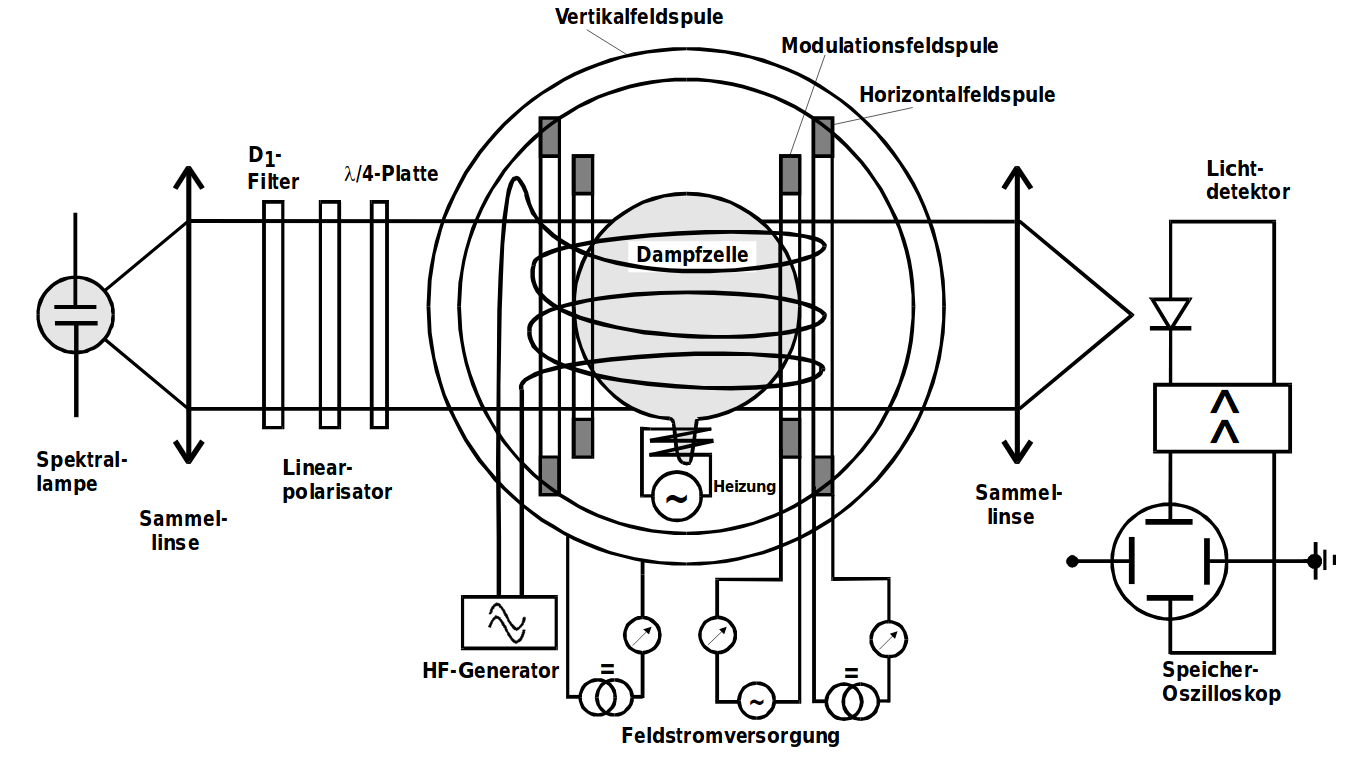
\includegraphics[width=0.7\textwidth]{content/pics/Aufbau.png}
  \caption{Verwendeter Versuchsaufbau \cite{anleitung}.}
  \label{Dur:Abb1}
\end{figure}

\subsection{Versuchsdurchführung}
Der Strahlengang wird durch schrittweises Einsetzen der optischen Elemente auf
maximale Intensität einjustiert und abgedeckt.
Es werden Sweep-Spulenfeld und Photostrom auf das Oszilloskop gegeben.
Durch drehen in Nord-Süd-Richtung und Variation des Vertikalfeldes wird das Erdmagnetfeld
kompensiert.
Sodann wird das Resonanzverhalten ausgemessen.
Durch einen Sinusgenerator wird das RF-Feld dabei in \SI{1}{\kilo\hertz}-Schritten
zwischen \SI{100}{\kilo\hertz} und \SI{1}{\mega\hertz} gesteigert.
Bei Frequenzen über \SI{200}{\kilo\hertz} wird der Sweep-Bereich durch das horizontale
Feld auf die Resonanzen verschoben, der Spulenstrom wird am Potentiometer abgelesen.
Es treten Resonanzen für beide Isotope auf, das Oszilloskop wird im XY-Modus
betrieben.
In einem zweiten Schritt wird durch Anlegen einer zusätzlichen Rechteckspannung
das Feld an- und ausgeschaltet.
Die Frequenz wird dabei auf die erste Resonanzstelle eingestellt.
Dabei wird der zeitliche Verlauf des Signals beobachtet, das Oszilloskop also
im YT-Modus betrieben und die zusätzliche Modulation wird durch Mittelung
auf dem Oszilloskop herausgerechnet.
Dies wird für beide Flanken des Signals und beide Isotope getan, wobei für die
steigende Flanke ein Bild aufgenommen und für das an der abfallenden Flanke
entstehenden Schwingverhalten die Periodendauer bestimmt wird.
